
\begin{figure}
    \centering
    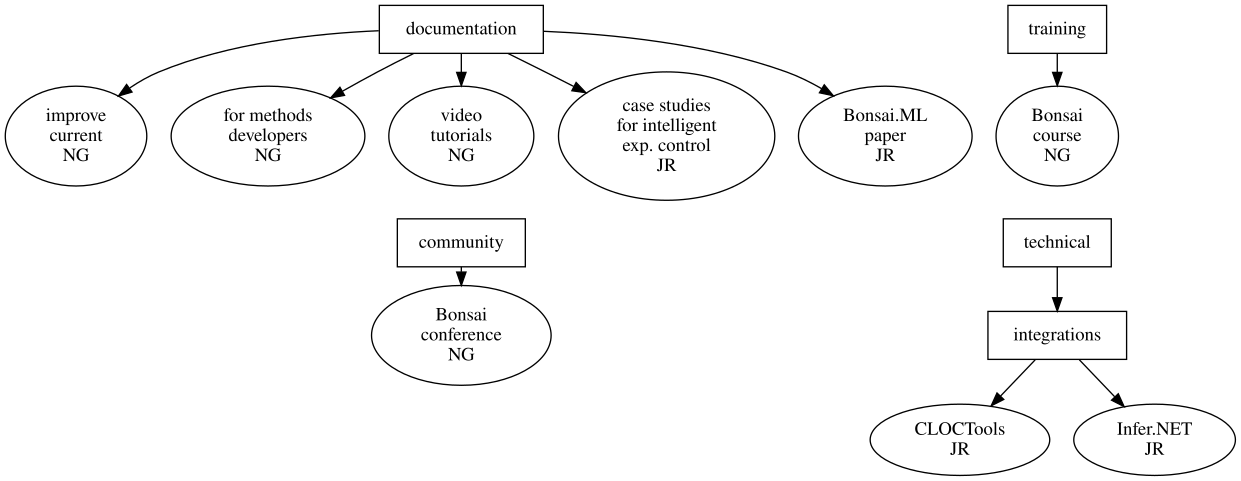
\includegraphics[width=6in]{activitiesGraphs/activities_larger.png}
    \caption{Proposed activities. See text for details.}
\end{figure}

Since most experimental neuroscientists currently using Bonsai are not highly
skilled in machine learning, to maximise the impact of Bonsai.ML, we need to
invest extra efforts on documentation, training and community building.
%
We add critical functionality to Bonsai.ML and streamline probabilistic
inference by integrating two packages.

\paragraph{1: Documentation} \textbf[Provide more examples] on the application
of the already integrated ML methods to new types of behavioural and neural
data. \textbf{Include video tutorials} on the use of the Bonsai.ML package.
\textbf{Add documentation for methods developers} as the current one is
targeted to Bonsai.ML users. \textbf{create case studies} for intelligent
experimental control in Bonsai. \textbf{Publish a first Bonsai.ML paper} as
companion papers substantially increases the adoption of software packages
\citep{lopesEtAl15,guilbeaultEtAl21}.

\paragraph{2: Training} Organise Bonsai course with Bonsai.ML module.

\paragraph{3: Community} Adoption of Bonsai.ML will greatly increase if we do
demonstrate the impact of Bonsai.ML for solving important neuroscience
problems.
%
We will collaborate with experimental neuroscientists to help them solve
relevant problems in intelligent experimental control.

\paragraph{Technical} Integrate into Bonsai the probabilistic programming
language Infer.NET\footnote[6]{https://dotnet.github.io/infer/} and tools for
close-loop control of neural activity,
ClocTools\footnote[7]{https://dotnet.github.io/infer/}.
